% ---------------------------------------------------------------------------
% Author guideline and sample document for EG publication using LaTeX2e input
% D.Fellner, v1.13, Jul 31, 2008

\documentclass{egpubl}
\usepackage{eurovis2019}

% --- for  Annual CONFERENCE
% \ConferenceSubmission   % uncomment for Conference submission
% \ConferencePaper        % uncomment for (final) Conference Paper
% \STAR                   % uncomment for STAR contribution
% \Tutorial               % uncomment for Tutorial contribution
% \ShortPresentation      % uncomment for (final) Short Conference Presentation
% \Areas                  % uncomment for Areas contribution
% \MedicalPrize           % uncomment for Medical Prize contribution
% \Education              % uncomment for Education contribution
% \Poster                 % uncomment for Poster contribution
% \DC                     % uncomment for Doctoral Consortium
%
% --- for  CGF Journal
% \JournalSubmission    % uncomment for submission to Computer Graphics Forum
% \JournalPaper         % uncomment for final version of Journal Paper
%
% --- for  CGF Journal: special issue
% \SpecialIssueSubmission    % uncomment for submission to , special issue
% \SpecialIssuePaper         % uncomment for final version of Computer Graphics Forum, special issue
%                          % EuroVis, SGP, Rendering, PG
% --- for  EG Workshop Proceedings
% \WsSubmission      % uncomment for submission to EG Workshop
% \WsPaper           % uncomment for final version of EG Workshop contribution
% \WsSubmissionJoint % for joint events, for example ICAT-EGVE
% \WsPaperJoint      % for joint events, for example ICAT-EGVE
% \Expressive        % for SBIM, CAe, NPAR
% \DigitalHeritagePaper
% \PaperL2P          % for events EG only asks for License to Publish

% --- for EuroVis 
% for full papers use \SpecialIssuePaper
% \STAREurovis   % for EuroVis additional material 
\EuroVisPoster % for EuroVis additional material 
% \EuroVisShort  % for EuroVis additional material

 \electronicVersion % can be used both for the printed and electronic version

% !! *please* don't change anything above
% !! unless you REALLY know what you are doing
% ------------------------------------------------------------------------

% for including postscript figures
% mind: package option 'draft' will replace PS figure by a filename within a frame
\ifpdf \usepackage[pdftex]{graphicx} \pdfcompresslevel=9
\else \usepackage[dvips]{graphicx} \fi

\PrintedOrElectronic

% prepare for electronic version of your document
\usepackage{t1enc,dfadobe}

\usepackage{egweblnk}
\usepackage{cite}

% For backwards compatibility to old LaTeX type font selection.
% Uncomment if your document adheres to LaTeX2e recommendations.
% \let\rm=\rmfamily    \let\sf=\sffamily    \let\tt=\ttfamily
% \let\it=\itshape     \let\sl=\slshape     \let\sc=\scshape
% \let\bf=\bfseries

% end of prologue
% ---------------------------------------------------------------------
% EG author guidelines plus sample file for EG publication using LaTeX2e input
% D.Fellner, v2.02, Jan 25, 2017


\title[ForumExplorer]%
      {ForumExplorer: A Forested View for Online Threaded Conversations}

% for anonymous conference submission please enter your SUBMISSION ID
% instead of the author's name (and leave the affiliation blank) !!
% for final version: please provide your *own* ORCID in the brackets following \orcid; see https://orcid.org/ for more details.
\author[A. McNutt \& G. Kindlmann]
{\parbox{\textwidth}{\centering A. McNutt, IEEE student member, \& G. Kindlmann
%        S. Spencer$^2$\thanks{Chairman Siggraph Publications Board}  
        }
        \\
% For Computer Graphics Forum: Please use the abbreviation of your first name.
{\parbox{\textwidth}{\centering Department of Computer Science, University of Chicago
%        $^2$ Another Department to illustrate the use in papers from authors
%             with different affiliations
       } 
}
}
% ------------------------------------------------------------------------

% if the Editors-in-Chief have given you the data, you may uncomment
% the following five lines and insert it here
%
% \volume{36}   % the volume in which the issue will be published;
% \issue{1}     % the issue number of the publication
% \pStartPage{1}      % set starting page


%-------------------------------------------------------------------------
\begin{document}

\teaser{
 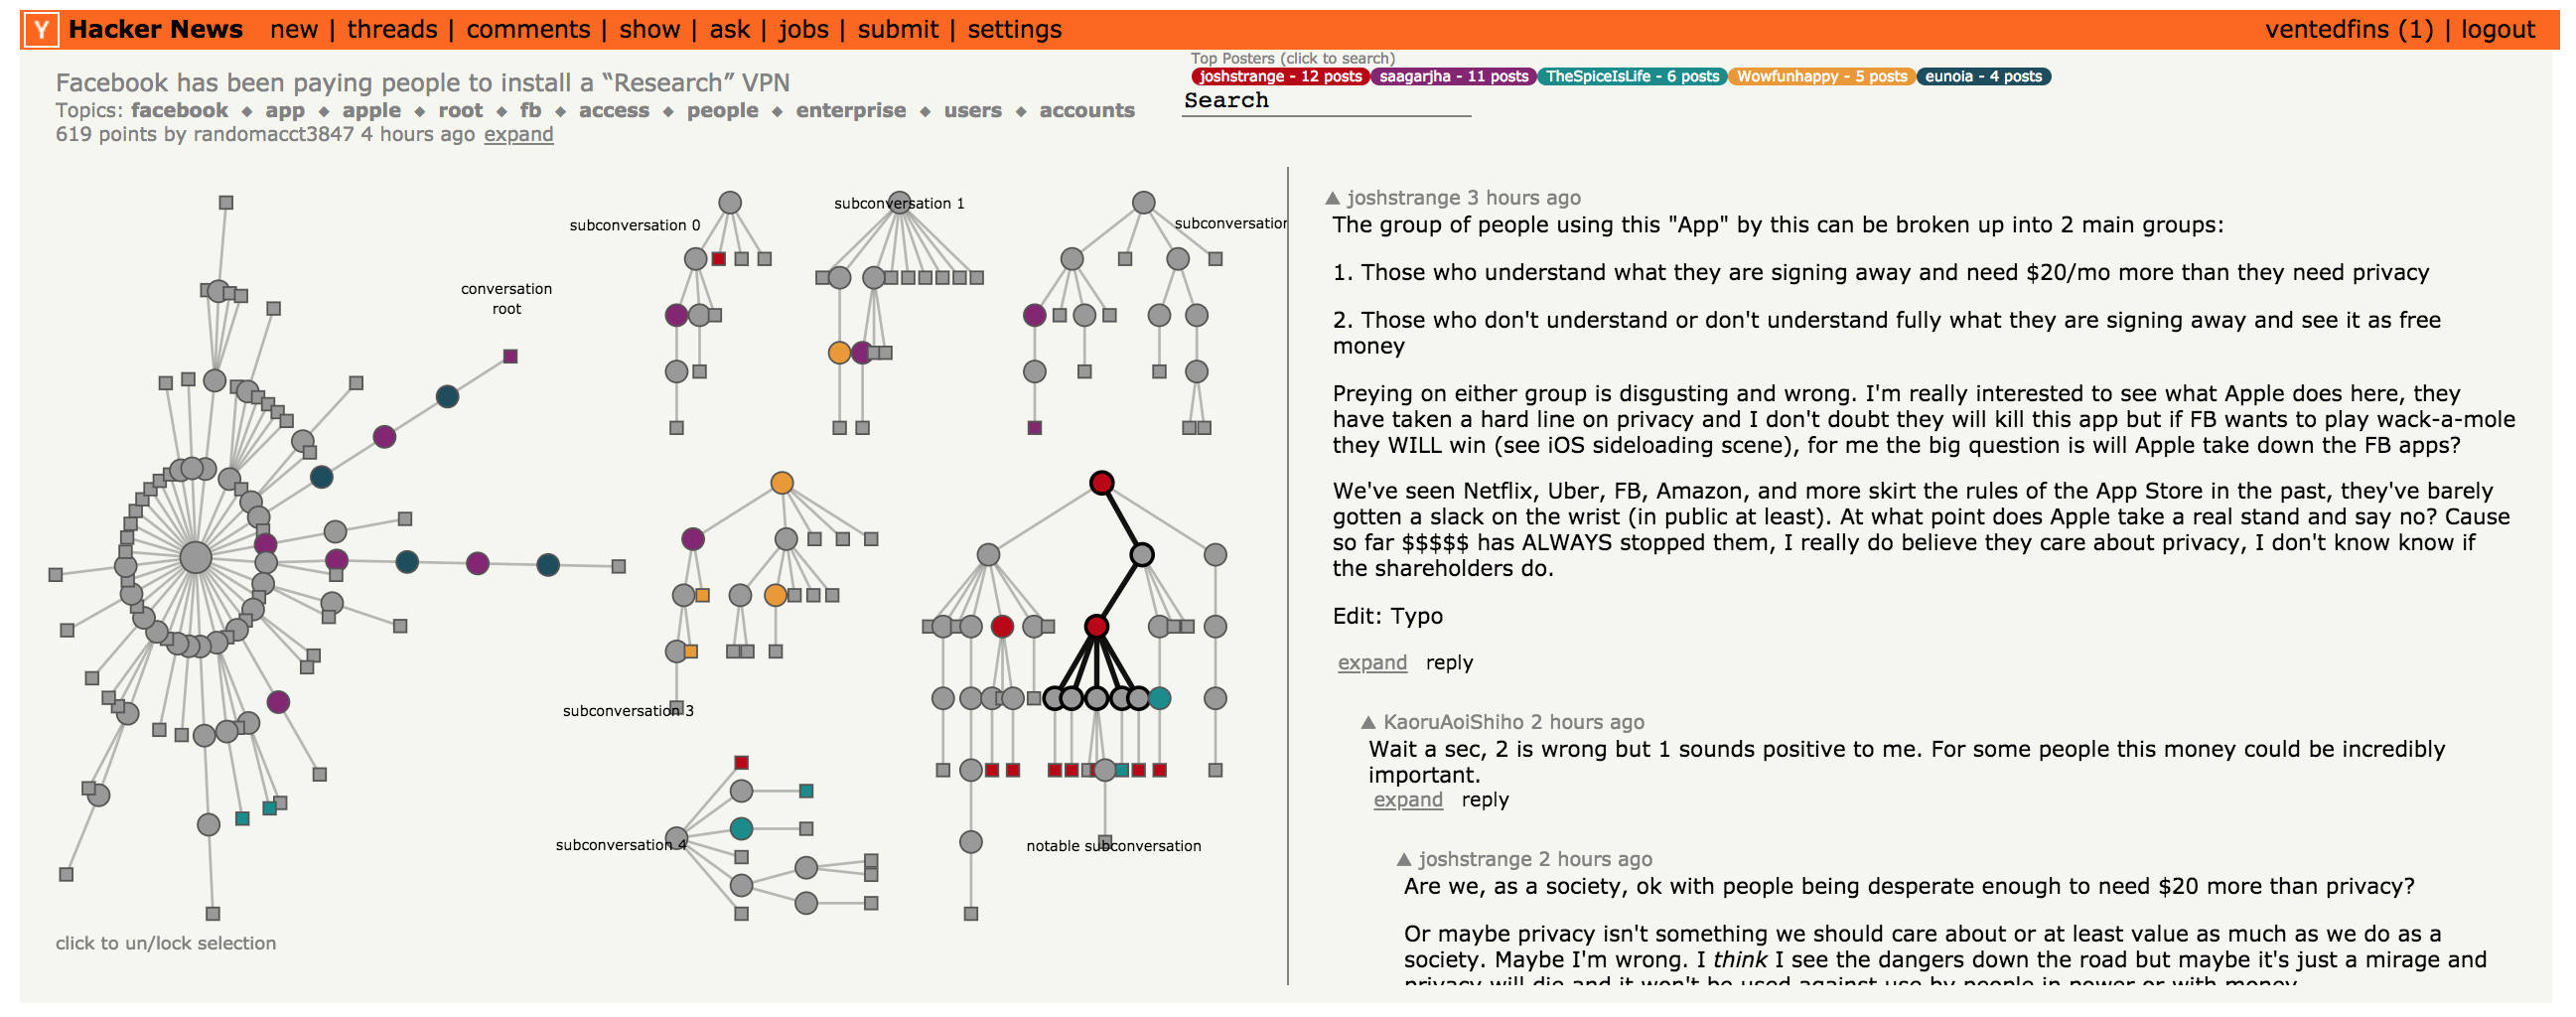
\includegraphics[width=\linewidth]{images/teaser.png}
 \centering
  \caption{New EG Logo}
\label{fig:teaser}
}

\maketitle
%-------------------------------------------------------------------------
\begin{abstract}
   The ABSTRACT is to be in fully-justified italicized text, 
   between two horizontal lines,
   in one-column format, 
   below the author and affiliation information. 
   Use the word ``Abstract'' as the title, in 9-point Times, boldface type, 
   left-aligned to the text, initially capitalized. 
   The abstract is to be in 9-point, single-spaced type.
   The abstract may be up to 3 inches (7.62 cm) long. \\
   Leave one blank line after the abstract, 
   then add the subject categories according to the ACM Classification Index 
%-------------------------------------------------------------------------
%  ACM CCS 1998
%  (see http://www.acm.org/about/class/1998)
% \begin{classification} % according to http:http://www.acm.org/about/class/1998
% \CCScat{Computer Graphics}{I.3.3}{Picture/Image Generation}{Line and curve generation}
% \end{classification}
%-------------------------------------------------------------------------
%  ACM CCS 2012
   (see http://www.acm.org/about/class/class/2012)
%The tool at \url{http://dl.acm.org/ccs.cfm} can be used to generate
% CCS codes.
%Example:
\begin{CCSXML}
<ccs2012>
<concept>
<concept_id>10010147.10010371.10010352.10010381</concept_id>
<concept_desc>Computing methodologies~Collision detection</concept_desc>
<concept_significance>300</concept_significance>
</concept>
<concept>
<concept_id>10010583.10010588.10010559</concept_id>
<concept_desc>Hardware~Sensors and actuators</concept_desc>
<concept_significance>300</concept_significance>
</concept>
<concept>
<concept_id>10010583.10010584.10010587</concept_id>
<concept_desc>Hardware~PCB design and layout</concept_desc>
<concept_significance>100</concept_significance>
</concept>
</ccs2012>
\end{CCSXML}

\ccsdesc[300]{Computing methodologies~Collision detection}
\ccsdesc[300]{Hardware~Sensors and actuators}
\ccsdesc[100]{Hardware~PCB design and layout}


\printccsdesc   
\end{abstract}





%-------------------------------------------------------------------------
\section{Introduction}


%%%
%%% Figure 1
%%%
\begin{figure}[htb]
  \centering
  % the following command controls the width of the embedded PS file
  % (relative to the width of the current column)
  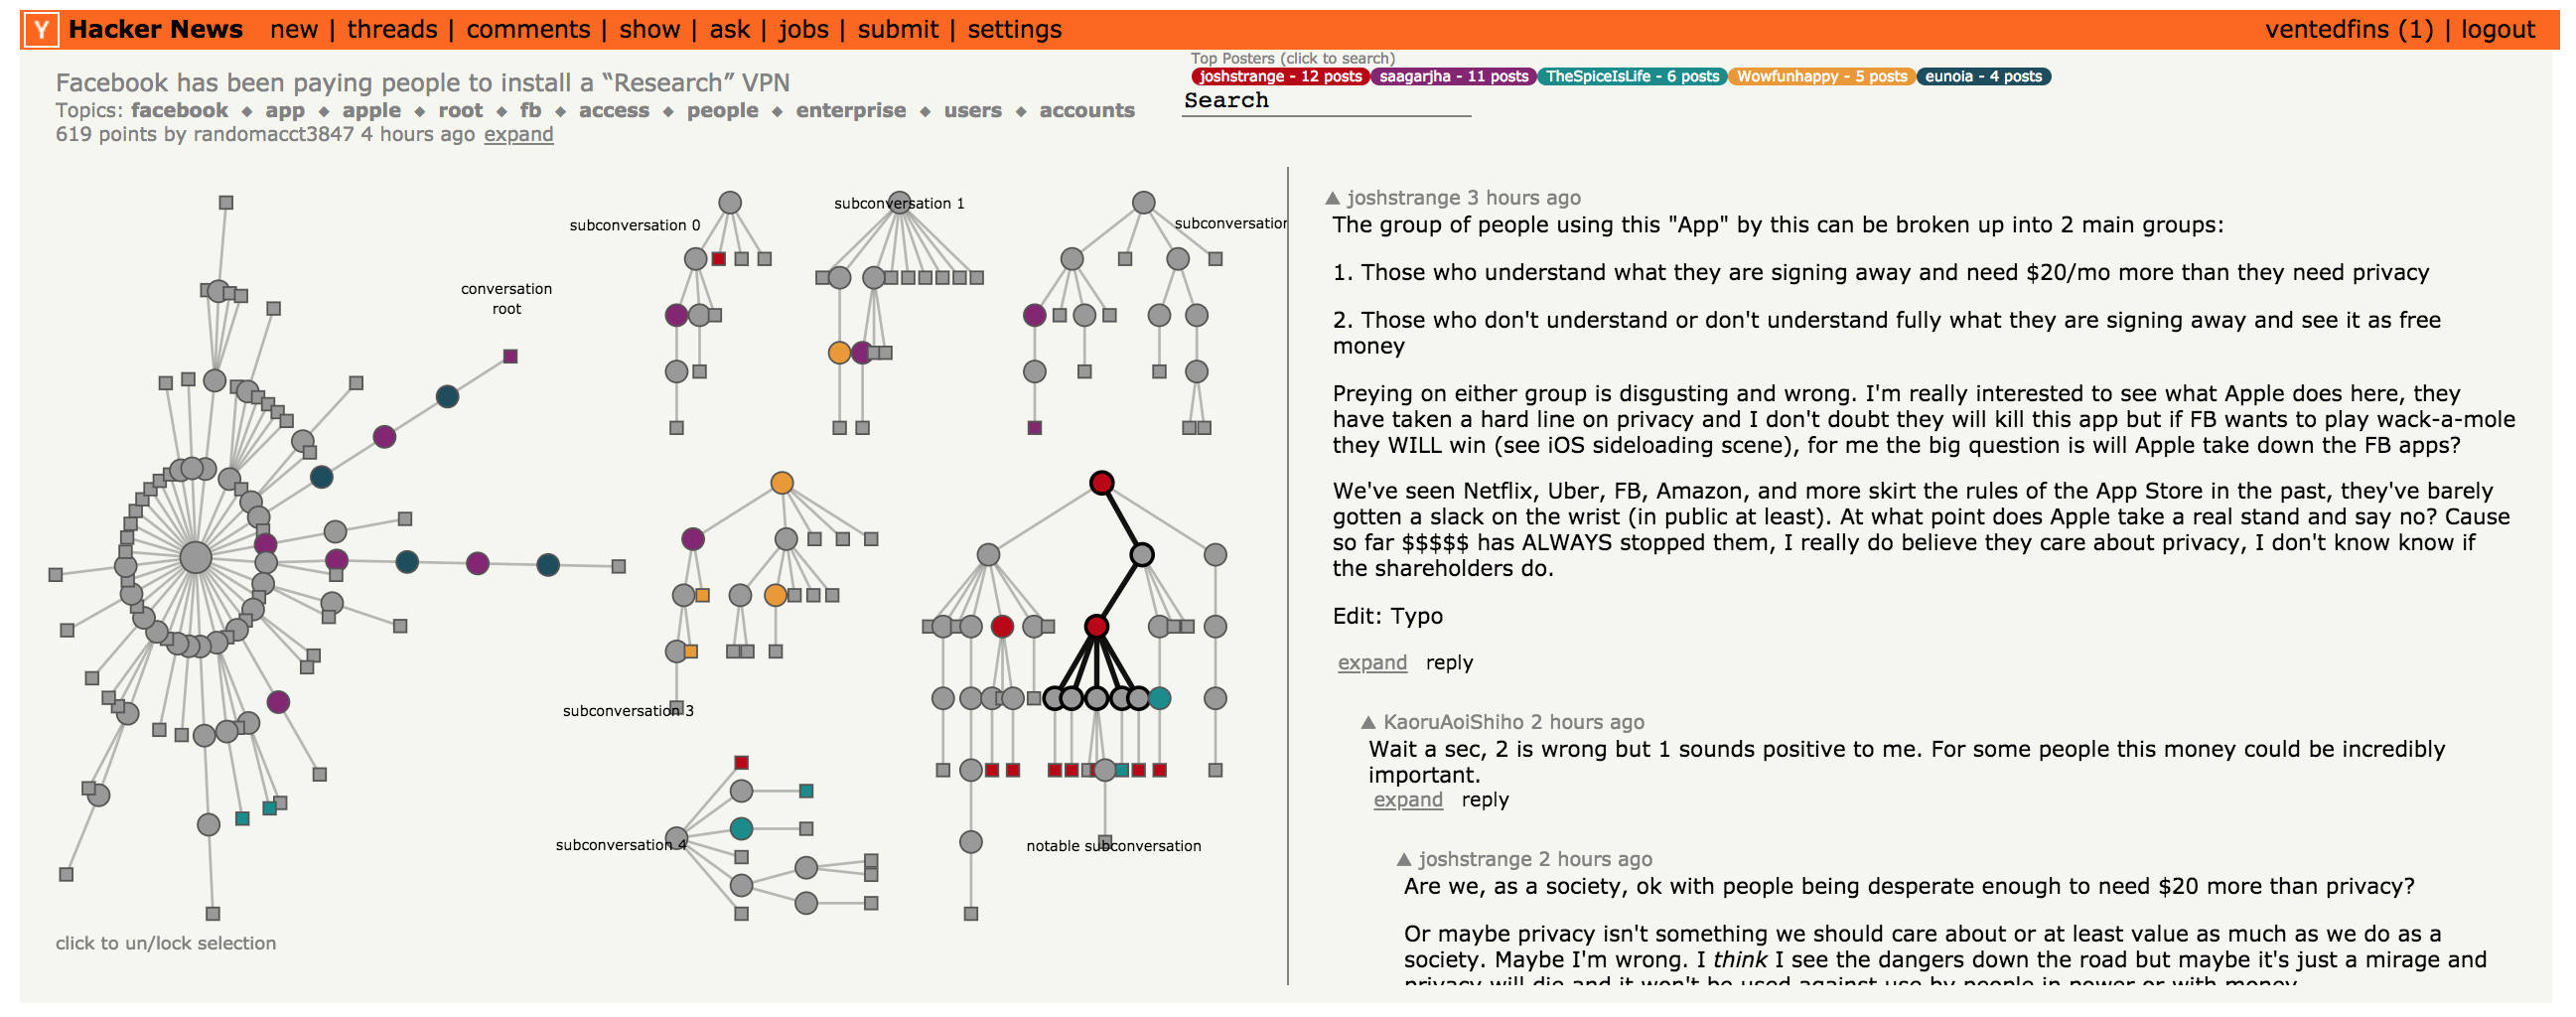
\includegraphics[width=.8\linewidth]{images/teaser.png}
  % replacing the above command with the one below will explicitly set
  % the bounding box of the PS figure to the rectangle (xl,yl),(xh,yh).
  % It will also prevent LaTeX from reading the PS file to determine
  % the bounding box (i.e., it will speed up the compilation process)
  % \includegraphics[width=.95\linewidth, bb=39 696 126 756]{sampleFig}
  %
  \parbox[t]{.9\columnwidth}{\relax
           For all figures please keep in mind that you \textbf{must not}
           use images with transparent background! 
           }
  %
  \caption{\label{fig:firstExample}
           Here is a sample figure.}
\end{figure}

example citation \cite{FolDamFeiHug.etal93}

%-------------------------------------------------------------------------
\subsection{Conclusions}

%-------------------------------------------------------------------------

%\bibliographystyle{eg-alpha}
\bibliographystyle{eg-alpha-doi}

\bibliography{forum-bib}

\end{document}

